\newpage
\begin{center}
    \Huge{\textbf{\underline{Chapter 2: Design Pattern}}}
\end{center}

\setcounter{section}{0}

\vspace{0.35cm}

\section{Design Pattern}

\begin{prettyBox}{Definition}{myblue}
A design pattern describes \textbf{proven} and \textbf{abstract} solutions  
to \textbf{recurring} problems in software design.
\end{prettyBox}


\vspace{0.35cm}
\begin{prettyBox}{Why Proven}{red}
Proven solutions have been tested on real projects, ensuring reliability and effectiveness.
\end{prettyBox}

\vspace{0.35cm}
\begin{prettyBox}{Why Abstract}{red}
Abstract solutions can be adapted and customized to meet specific needs.
\end{prettyBox}

\vspace{0.35cm}
\begin{prettyBox}{Why Recurring}{red}
We want model for recurring problems to address patterns in design problems that repeat across different contexts.
\end{prettyBox}


\vspace{0.5cm}
\section{Categories}
\begin{prettyBox}{Categories}{myblue}
The first influential book on design patterns, \textbf{Design Patterns: Elements of Reusable
Object-Oriented Software} by the "Gang of Four" (Erich Gamma, Richard Helm,
Ralph Johnson, and John Vlissides), was published in its second edition in 1995.
It presents a collection of 23 design patterns, classified into three categories.
\end{prettyBox}

\vspace{0.75cm}


\subsection{Creational Design Patterns (5 from the Gang of Four Collection)}
\begin{prettyBox}{Creational}{myblue}
Describes how to fix problems of class instantiations.
\end{prettyBox}

\newpage

\subsection{Structural Design Patterns (7 from the Gang of Four Collection)}
\begin{prettyBox}{Structural Design Pattern}{myblue}
Describes how to structure classes with a minimum of dependencies.
\end{prettyBox}

\vspace{0.25cm}

\subsection{Behavioral Design Patterns (11 from the Gang of Four Collection)}
\begin{prettyBox}{Behavioral Design Pattern}{myblue}
Describe how to ensure a specific behavior of the application.
\end{prettyBox}


\vspace{0.25cm}
\begin{prettyBox}{Note}{red}
The design patterns from the "Gang of Four" are intended for
object-oriented design.
\end{prettyBox}

\vspace{0.5cm}

\section{Pros \& Cons}
\begin{prettyBox}{Pros \& Cons}{myblue}
\textbf{\underline{Pros}}
\begin{itemize}
    \item Solves recurring problems with proven and reliable solutions.
    \item Improves quality and speed.
    \item Design patterns provide a common language for communication between designers.
    \item Design patterns are independent of implementation languages and sufficiently generic (abstract) to be applied in various situations.
\end{itemize}

\textbf{\underline{Cons}}
\begin{itemize}
    \item Design patterns need to be mastered and thoroughly studied.
    \item Design patterns always require adaptation when applied.
    \item Design patterns can increase the complexity of simple solutions.
\end{itemize}

\end{prettyBox}

\vspace{0.25cm}

\begin{prettyBox}{Formalism Of A Design Pattern}{red}
The formalism of a design pattern (description of a design pattern) consists of:  
\begin{itemize}
    \item Name of the design pattern.  
    \item Addressed problem.  
    \item Proposed solution.  
    \item Other sections (pros \& cons, usage examples and context before and after usage, usage recommendations, etc.).  
\end{itemize}
\end{prettyBox}

\vspace{0.5cm}

\begin{prettyBox}{Principles Favored by Design Patterns}{red}
Design patterns of the "Gang of Four" promote good design (low coupling,  
high cohesion, etc.) and two principles:  
\begin{itemize}
    \item \textbf{Principle\(_1\)}: Favor composition over inheritance (favor \(\neq\) replace)  
    \item \textbf{Principle\(_2\)}: Clients interact with the abstractions rather  
        than the implementations  
\end{itemize}
\end{prettyBox}

\vspace{1cm}
\section{Some Design Pattern}

\subsection{Singleton Creational Design Pattern}
\begin{prettyBox}{Singleton}{myblue}
The Singleton is a creational design pattern that limits the number of instantiations to
a single object and makes it globally accessible.
\end{prettyBox}

\begin{center}
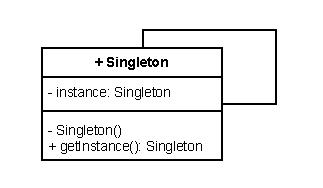
\includegraphics[width=0.55\textwidth]{Chapters/DesignPattern/Singleton/single.drawio.pdf}
\end{center}

\begin{prettyBox}{Explication}{myblue}
We first initialize a static private attribut called instance to null , when ever we want to get instance of singleton
we call the public static method getInstance that checks if instance is null if yes it will call the private constructor
and in either case it returns the instance 
\end{prettyBox}

\newpage
\subsubsection*{\underline{Java Code:}}

\lstinputlisting[style=javastyle]{Chapters/DesignPattern/Singleton/S1/Singleton.java}

\vspace{0.5cm}
\lstinputlisting[style=javastyle]{Chapters/DesignPattern/Singleton/S1/Main.java}


\subsubsection*{\underline{Output:}}
\begin{lstlisting}[style=cmd]
Instance Of Singleton
\end{lstlisting}

\vspace{0.5cm}

\begin{prettyBox}{Thread Safe}{red}
This implementation isn't thread-safe. If two or more threads  
run \texttt{getInstance()}, they may call the constructor at the same time,  
creating multiple objects and violating the Singleton pattern.
\end{prettyBox}

\newpage

\textbf{\underline{Java Code:}}
\lstinputlisting[style=javastyle]{Chapters/DesignPattern/Singleton/S1/ThreadMain.java}

\vspace{0.5cm}

\textbf{\underline{Output:}}
\begin{lstlisting}[style=cmd]
Running on thread: Thread-1
Running on thread: Thread-0
Running on thread: Thread-2
Instance Of Singleton
Instance Of Singleton
\end{lstlisting}

\vspace{1cm}
\begin{prettyBox}{How To Make It Thread-Safe}{myblue}
As we can see, in a multi-threaded scenario, the current implementation
fails to maintain a single instance. To fix that, we will use 
\texttt{volatile} and \texttt{synchronized} keywords:
\begin{itemize}
    \item \texttt{synchronized}: Ensures that the function, class, instance,
        or block of code is executed by only one thread at a time (mutual exclusion).
    \item \texttt{volatile}: Ensures the variable is stored in the main memory
        (RAM) rather than the cache memory. It is used to prevent two issues:
        \begin{itemize}
            \item \textbf{Memory cache inconsistency}: Sometimes, a thread may change a variable in its
                local memory cache, but OS protocols may not propagate the update to the other 
                thread’s cache in time, causing other threads to read an outdated value.
        \item \textbf{Partially initialized object}: A thread might start creating the instance, 
                but another thread checks if the instance is not null, which is true, and 
                returns an incomplete object because the first thread hasn’t finished its creation, 
                potentially crashing the application.
        \end{itemize}
\end{itemize}
\end{prettyBox}

\newpage
\textbf{\underline{Java Code:}}
\lstinputlisting[style=javastyle]{Chapters/DesignPattern/Singleton/S1/ThreadSingle1.java}

\vspace{0.5cm}

\textbf{\underline{Output:}}
\begin{lstlisting}[style=cmd]
Running on thread: Thread-2
Running on thread: Thread-1
Instance Of Singleton
Running on thread: Thread-0
\end{lstlisting}

\vspace{1cm}

\begin{prettyBox}{Optimization}{myblue}
The implementation is correct and thread-safe, but we can optimize it:
\begin{itemize}
    \item Add a check if \texttt{instance} is null before entering the \texttt{synchronized} block 
        to avoid unnecessary overhead and only enter the mutex when \texttt{instance} is null.
    \item Accessing main memory is slow, so we can use a local variable inside the 
        \texttt{getInstance()} function to reduce redundant memory reads.
\end{itemize}
\end{prettyBox}

\newpage
\textbf{\underline{Check If Null Before Synchronized Block:}}
\lstinputlisting[style=javastyle]{Chapters/DesignPattern/Singleton/S1/ThreadSingle3.java}

\vspace{1cm}

\textbf{\underline{Local Variable:}}
\lstinputlisting[style=javastyle]{Chapters/DesignPattern/Singleton/S1/ThreadSingle2.java}

\newpage
\null

\begin{prettyBox}{Breaking With Reflection}{myblue}
Even though the current implementation is thread-safe it is weak against
reflection as we can fetch constrcutor of the \texttt{Singelton} and set 
them as \texttt{public} at run time.
\end{prettyBox}

\vspace{1cm}

\textbf{\underline{Reflection}}
\vspace{0.1cm}

\lstinputlisting[style=javastyle]{Chapters/DesignPattern/Singleton/break.java}

\vspace{1cm}

\textbf{\underline{Output}}
\vspace{0.1cm}
\begin{lstlisting}[style=cmd]
Instance Of Singleton
Instance Of Singleton
804564176
1421795058
\end{lstlisting}





\newpage
\subsection{Composite Structural Design Pattern}
\begin{prettyBox}{Composite}{myblue}
The Composite pattern is a structural design pattern that imposes a
hierarchical tree structure, consisting of simple elements and composite elements, and 
Allows manipulating different objects in a uniform way
\end{prettyBox}

\vspace{1cm}


\begin{center}
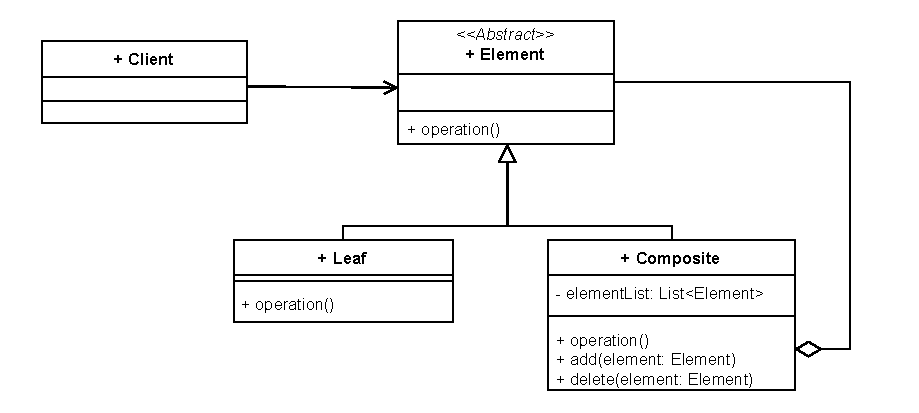
\includegraphics[height=0.22\textheight]{Chapters/DesignPattern/Composite/comp1.drawio.pdf}
\end{center}

\vspace{1cm}

\begin{prettyBox}{Explication}{myblue}
The Element class serves as an abstract parent class with an unimplemented method, operation().  
The Leaf class inherits from Element and overrides the operation() method to provide its specific implementation.  
Similarly, the Composite class also inherits from Element and implements operation(). However, it has an attribute that is a collection of Element objects.  
This design allows the collection to hold both simple elements (Leaf) and complex elements (Composite), organizing them into a tree structure.\\[0.1cm]
This abstraction provides a unified interface and defines a common behavior (\texttt{operation()}) 
for all elements, allowing the client class to manipulate them uniformly.
\end{prettyBox}

\vspace{0.5cm}
\begin{prettyBox}{Note}{red}
Element can be an abstract class or an interface both implementations are valid.
\end{prettyBox}

\newpage
\textbf{\underline{Graphical Representation Of The Composite}}

\vspace{0.25cm}
\begin{center}
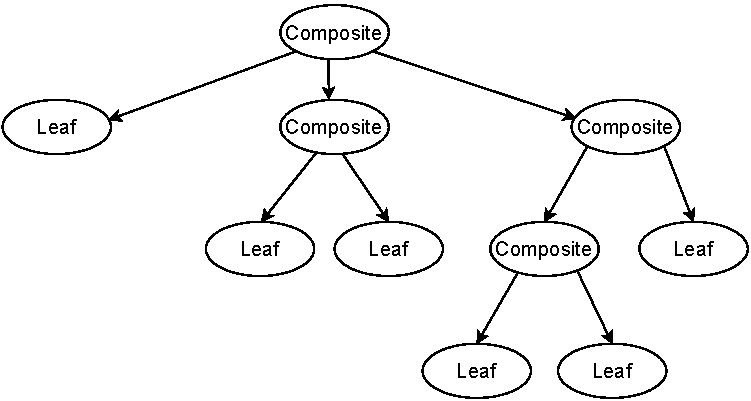
\includegraphics[height=0.3\textheight]{Chapters/DesignPattern/Composite/tree.drawio.pdf}
\end{center}



\vspace{1cm}
\subsubsection*{\underline{Java Code:}}

\lstinputlisting[style=javastyle]{Chapters/DesignPattern/Composite/C1/Element.java}

\vspace{0.5cm}
\lstinputlisting[style=javastyle]{Chapters/DesignPattern/Composite/C1/Leaf.java}
\newpage
\null
\vspace{1cm}
\lstinputlisting[style=javastyle]{Chapters/DesignPattern/Composite/C1/Composite.java}

\newpage
\lstinputlisting[style=javastyle]{Chapters/DesignPattern/Composite/C1/Main.java}

\vspace{1cm}

\subsubsection*{\underline{Output:}}
\begin{lstlisting}[style=cmd]
Leaf Operation
Leaf Operation
Composite Operation


Leaf
Leaf

 Composite
  Leaf
   Composite
    Leaf
    Leaf
\end{lstlisting}


\newpage

\subsection{Observer Behavioral Design Pattern}
\begin{prettyBox}{Observer}{myblue}
The Observer pattern consists of two parties: the \textbf{Subject} and the \textbf{Observers}:
\begin{itemize}
    \item \textbf{Subject}: Represents data that is prone to change state at runtime. It notifies the \textbf{Observers} of any changes.
    \item \textbf{Observers}: Are external class interested in the \textbf{Subject} and trigger actions based on its state.
\end{itemize}
\end{prettyBox}

\vspace{1cm}


\begin{center}
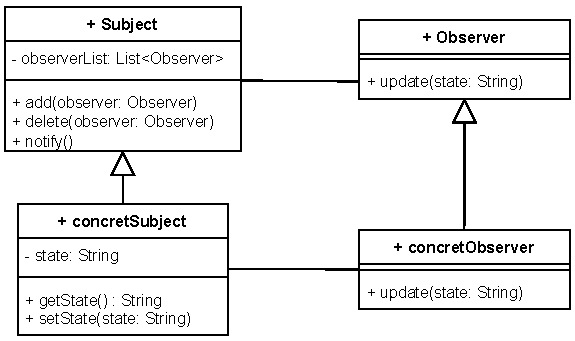
\includegraphics[height=0.35\textheight]{Chapters/DesignPattern/Observer/obs1.drawio.pdf}
\end{center}

\vspace{1cm}

\begin{prettyBox}{Explication}{myblue}
The \textbf{Observer} is an abstract class that defines an unimplemented method, \texttt{update()},
which is executed each time the state changes.

\vspace{0.25cm}
The \textbf{Subject} is also an abstract class,
which maintains a collection of observers and declares unimplemented methods:
\begin{itemize}
    \item  \texttt{add(observer)} : Add new observer to the list.
    \item \texttt{delete(observer)} : Remove an existing from the list.
    \item \texttt{notify()}: Loops through all the observer of the list and calls their \texttt{update()} method .
\end{itemize}

\vspace{0.25cm}
A \textbf{ConcreteObserver} inherits from \textbf{Observer} , holds reference of \textbf{concreteSubject} implements the 
\texttt{update()} method, along with a new method \texttt{checkState()} that calls the \texttt{getState()}
invoked within \texttt{update()}.

\vspace{0.25cm}
A \textbf{ConcreteSubject} inherits from \textbf{Subject}, overrides all unimplemented
methods, and includes a state attribute with its getter and setter. Whenever the setter is 
called, the \texttt{notify()} method is invoked within its body to ensure that all 
observers are updated.
\end{prettyBox}


\newpage

\begin{prettyBox}{Note}{red}
Subject and observer can be interfaces too.
\end{prettyBox}

\vspace{0.5cm}

\subsubsection*{\underline{Java Code:}}

\lstinputlisting[style=javastyle]{Chapters/DesignPattern/Observer/O1/Observer.java}

\vspace{1cm}
\lstinputlisting[style=javastyle]{Chapters/DesignPattern/Observer/O1/Subject.java}

\vspace{1cm}
\lstinputlisting[style=javastyle]{Chapters/DesignPattern/Observer/O1/concretObserver.java}

\newpage
\lstinputlisting[style=javastyle]{Chapters/DesignPattern/Observer/O1/concretSubject.java}

\vspace{1cm}

\lstinputlisting[style=javastyle]{Chapters/DesignPattern/Observer/O1/Main.java}

\subsubsection*{\underline{Output:}}
\begin{lstlisting}[style=cmd]
Setting state to State 1
Observer Alice New State : State 1
Observer Bob New State : State 1
Setting state to State 2
Observer Bob New State : State 2
Setting state to State
Observer Bob New State : State
\end{lstlisting}

\newpage

\textbf{\underline{Example :}}\\[0.15cm]
An application presents the data points (a, b, c) in three formats: table, a histogram, and a pie chart as shown below:

\begin{center}
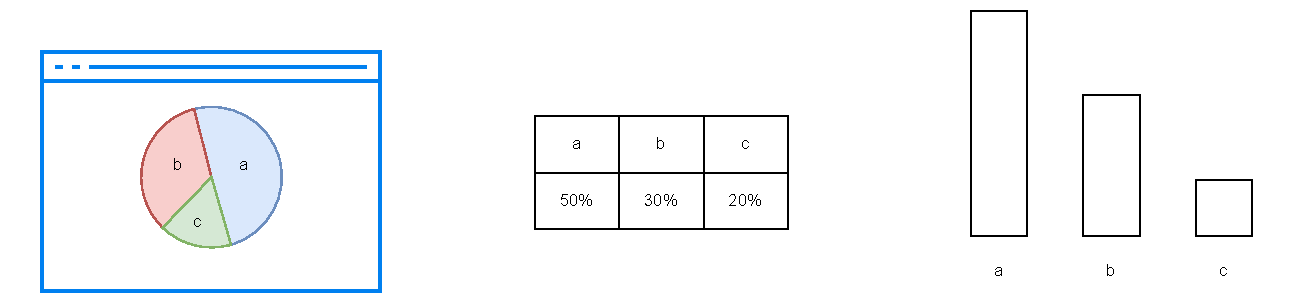
\includegraphics[width=0.85\textwidth]{Chapters/DesignPattern/Observer/ex1.drawio.pdf}
\end{center}

\vspace{0.5cm}

\begin{center}
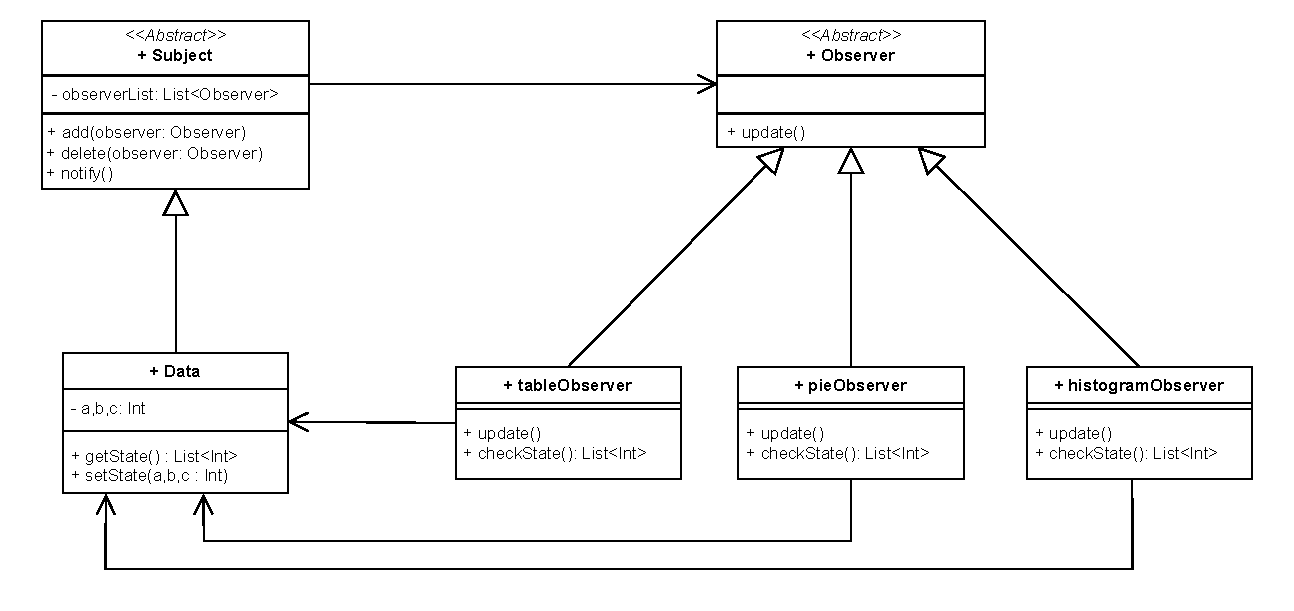
\includegraphics[width=0.85\textwidth]{Chapters/DesignPattern/Observer/obs.drawio.pdf}
\end{center}

\vspace{0.5cm}

\begin{prettyBox}{Explication}{myblue}
    \begin{itemize}
        \item The data elements \(a\), \(b\) and \(c\) are subject to change and thus constitute the \textbf{subject}. 
        \item The views \texttt{table}, \texttt{pie chart} and \texttt{histogram} are external classes that are interested to the subject’s state 
    and must update whenever it changes, making them \textbf{observers}.
    \end{itemize}
\end{prettyBox}


\newpage

\subsection{Strategy Behavioral Design Pattern}
\begin{prettyBox}{Strategy}{myblue}
The Strategy pattern consists of two parties: the \textbf{Context} and the \textbf{Strategies}:
\begin{itemize}
\item \textbf{Context}: Represents the class that users will interact with to choose the needed behavior at runtime
\item \textbf{Strategies}: Are all the interchangeable behavior classes a user might choose
\end{itemize}
To say Strategy is implemented correctly, the user must be able to select any behavior possible. The Strategy pattern allows us to separate the object from its behaviors and to make them interchangeable and selectable at runtime.
\end{prettyBox}

\vspace{1cm}


\begin{center}
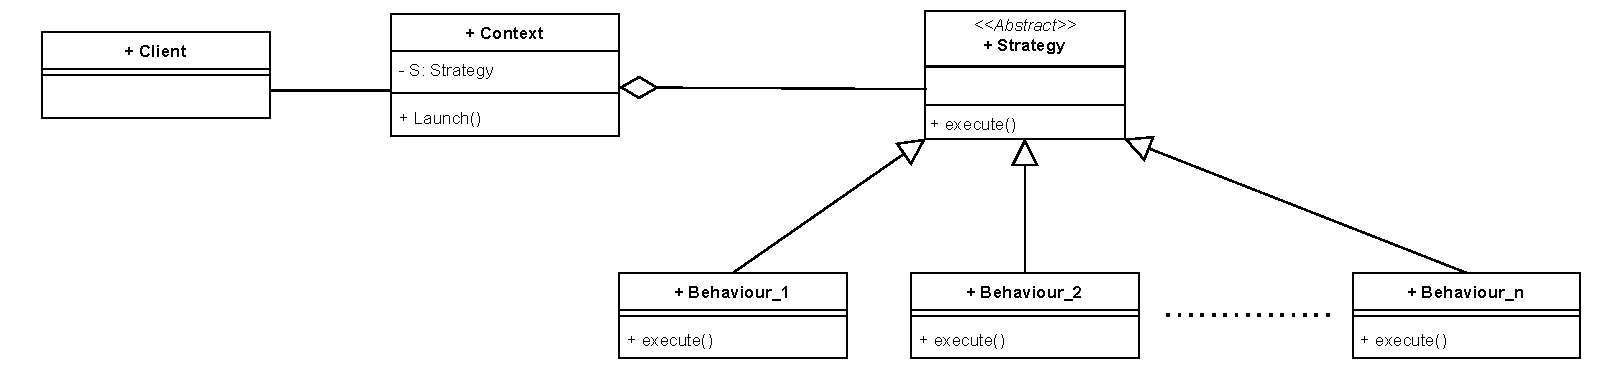
\includegraphics[height=0.15\textheight]{Chapters/DesignPattern/Strategy/str1.drawio.pdf}
\end{center}

\vspace{1cm}

\begin{prettyBox}{Explication}{myblue}
The \textbf{Strategy} is an abstract class that defines an unimplemented method, \texttt{execute()}, which is executed when the user chooses a behaviour at runtime.
\vspace{0.25cm}
The \textbf{Behaviour\(_i\)} are concrete classes that extend the \textbf{Strategy} class and implements the \texttt{execute()} method. 
They represent the different interchangeable behaviours a user might choose.
\vspace{0.25cm}
A \textbf{Context} is a class that the user will interact with to choose the needed behaviour. It holds a reference to a \textbf{Strategy} object
and has a method \texttt{Launch()} that will call the strategy's \texttt{execute()} method according to the user's choice. 
The context can switch between different strategies at runtime by changing which concrete behaviour implementation it references.
\end{prettyBox}

\vspace{0.25cm}

\begin{prettyBox}{Note}{red}
Strategy can be an interface.
\end{prettyBox}

\vspace{0.5cm}
\subsubsection*{\underline{Java Code:}}

\lstinputlisting[style=javastyle]{Chapters/DesignPattern/Strategy/Code/Strategy.java}

\newpage
\lstinputlisting[style=javastyle]{Chapters/DesignPattern/Strategy/Code/Behaviour_1.java}

\vspace{1cm}
\lstinputlisting[style=javastyle]{Chapters/DesignPattern/Strategy/Code/Behaviour_2.java}

\vspace{1cm}
\lstinputlisting[style=javastyle]{Chapters/DesignPattern/Strategy/Code/Behaviour_3.java}

\vspace{1cm}
\lstinputlisting[style=javastyle]{Chapters/DesignPattern/Strategy/Code/Context.java}

\newpage

\lstinputlisting[style=javastyle]{Chapters/DesignPattern/Strategy/Code/Main.java}

\subsubsection*{\underline{Output:}}
\begin{lstlisting}[style=cmd]
Press 1 For Strategy 1
Press 2 For Strategy 2
Press 3 For Strategy n
Press 0 to Quit
1
Behaviour_1 execute()
Press 1 For Strategy 1
Press 2 For Strategy 2
Press 3 For Strategy n
Press 0 to Quit
2
Behaviour_2 execute()
Press 1 For Strategy 1
Press 2 For Strategy 2
Press 3 For Strategy n
Press 0 to Quit
3
Behaviour_n execute()
Press 1 For Strategy 1
Press 2 For Strategy 2
Press 3 For Strategy n
Press 0 to Quit
0

\end{lstlisting}

\newpage

\textbf{\underline{Example :}}\\[0.15cm]
An application that computes the vertical speed of an element and taking account of gravity and friction.

\vspace{0.5cm}

\begin{center}
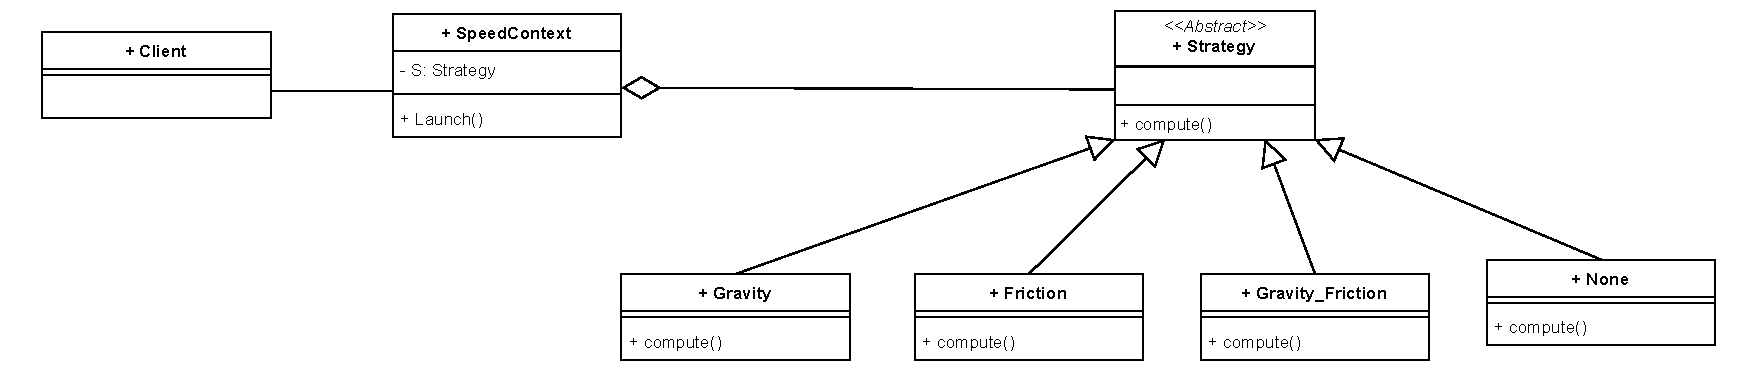
\includegraphics[width=0.85\textwidth]{Chapters/DesignPattern/Strategy/str2.drawio.pdf}
\end{center}

\vspace{0.5cm}

\begin{prettyBox}{Explication}{myblue}
    \begin{itemize}
        \item When computing vertical speed there are 4 cases : with gravity only , with firction only , both and none , all of these
            represents different strategies of our application , therefor each case will be a class extending \textbf{Strategy} class.
        \item The \textbf{speedContext} is the class user will interact with to choose the needed strategy at run time .
    \end{itemize}
\end{prettyBox}

